\subsubsection{Vorstellung des Amazon Dash Buttons}        
\label{sec:Vorstellung des Amazon Dash Buttons} 
Am 31.08.16 wurde der Amazon Dash Button offiziell in Deutschland exklusiv für Prime Mitglieder eingeführt (vgl. \cite{ONLINE.31.08.2016}).
Dabei handelt es sich um einem mit dem WLAN verbundenen Button, mit welchem sich zum Großteil Verbrauchsartikel per Knopfdruck bestellen lassen.
Jeder Button wird mit einem Produkt verknüpft, das während des Einrichtens ausgewählt wird.
Sollte nun das Produkt zur Neige gehen oder gar aufgebraucht sein, so kann der Nutzer den Button drücken und es wird sofort ein Bestellvorgang eingeleitet.
Weitere Interaktion seitens des Nutzers ist dabei nicht notwendig.
Der Dash Button wird über die Amazon App auf einem Android- oder iOS-Smartphone eingerichtet und verwaltet und funktioniert an allen Orten mit einer WLAN-Verbindung.
Sobald die Einrichtung abgeschlossen ist, wird eine Benachrichtigung (sofern aktiviert) an das Smartphone versendet, immer wenn eine Bestellung aufgegeben wurde. (vgl. \cite{.dash})
Zusätzlich verfügt der Button über einen Bestellschutz.
Mit dieser Funktion gibt der Dash Button keine Bestellung auf, bis die vorherige Bestellung geliefert wurde – egal wie oft der Dash Button gedrückt wird.
Der Amazon Dash Button ist in Deutschland für aktuell 4,99 \euro erhältlich (Stand: 17.05.17).
Jedoch wird dieser Preis mit der ersten Bestellung verrechnet, wodurch dem Kunden keine zusätzlichen Kosten entstehen.

\begin{figure}[!htb]
	\centering
	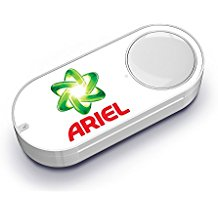
\includegraphics[scale=0.5]{Dash.jpg}
	\caption[Amazon Dash Button für Produkte von Ariel]{Amazon Dash Button für Produkte von Ariel,\\ Quelle: https://images-eu.ssl-images-amazon.com/images/I/41SMHhklQYL.\_AC\_US218\_.jpg}
\end{figure}

\subsubsection{Untersuchung des Amazon Dash Buttons}
\label{sec:Untersuchung des Amazon Dash Buttons}
Die Untersuchung des Amazon Dash Buttons bezieht sich nur auf dessen Funktionen.
Die Hardware wurde nicht analysiert, da diese bereits mehrfach, auch auf unterschiedlichen Websites analysiert wurde (vgl. \cite{.17.05.2017}\cite{.17.05.2017b})
Der Amazon Dash Button wird einem kleinen braunen Karton geliefert.
Dieser enthält neben dem Button noch 2 Dokumente, eine Gebrauchsanleitung und Sicherheitsinformationen.
Die Gebrauchsanleitung beschreibt nur den Download der Amazon App sowie die schritte, die notwendig sind um den Konfigurationsassistenten zu starten.
Die eigentlich Einrichtung läuft dann wie folgt ab:
Zuerst müssen WLAN und Bluetooth auf dem Gerät aktiviert werden.
Danach muss der Amazon Dash Button für ca. 6 Sekunden gedrückt werden, bis dieser Blau leuchtet.

\subsubsection{Verwendung des Amazon Dash Buttons im Projekt}
\label{sec:Verwendung des Amazon Dash Buttons im Projekt}
Der Amazon Dash Button konnte erfolgreich in das Projekt eingebunden werden. Hierbei waren jedoch ein paar Workarounds notwendig, welche in \ref{sec:Einbindung des Amazon Dash Buttons-1} näher ausgeführt werden. Dabei funktioniert der Dash Button genauso wie die selbst einwickelten Button.